\section{Population Analisys} \label{numbers}

\onehalfspacing

In order for this crowdsourcing network to be a useful service, certain population and active-user requirements must be met. Specifically, in order for the network to be used within a particular geographic area, the population density of autoinjector carriers must be high enough to make sharing their autoinjectors logistically possible within a reasonable amount of time. Based on this necessity, the following probabilistic measure is considered:\newline
%In addition, if the population density of autoinjector carriers in a particular area is high enough to make the creation of the network possible, there must be enough people registered on the network to make it useful. 
\begin{adjustwidth}{2.5em}{0pt}
    In the event that Person $X$ is looking for an autoinjector in Area $A$, what is the probability that there exists some Autoinjector Carrier $Y$ such that the distance between $X$ and $Y$ makes it possible for $Y$ to walk to $X$ faster than an ambulance could travel to $X$?
\end{adjustwidth}
% Given that there are $n$ registered users on the network in Area $A$, what is the probability that, in the event that Person $X$ is looking for an autoinjector carrier in Area $A$, there exists some \textit{registered} Autoinjector Carrier $R$ such that the distance between $X$ and $R$ makes it possible for $R$ to walk to $X$ faster than an ambulance could travel to $X$?
\noindent\newline This asks whether or not the creation of this network is possible based on the population densities of people who carry autoinjectors. This probability will be used to show that the network effect of sharing autoinjectors is, in fact, possible. We address this question in the following two sections.


\subsection{Autoinjectors Nearby} \label{autoinjectors-nearby}

Let $R$ be the event that Person $X$ is having an allergic reaction and needs an autoinjector in area $A$. Let the random variable $N$ be the number of autoinjector carriers nearby Person $X$ in Area $A$. In order to determine if a peer-to-peer network of autoinjectors is possible, we need to find the probability that there are at least $k$ autoinjector carriers nearby Person $X$, given that Person $X$ has a reaction in Area $A$. Thus, we are looking for $P(N \geq k|R)$. For purposes of simplicity, we will assume that Person $X$ having a reaction does not increase the probability that someone with an autoinjector nearby, and thus assume $N$ is independent of $R$. Thus, we are looking for the probability that there are at least $n$ people carrying autoinjectors in area $A$ at any given time, or
\begin{align*}
    P(N \geq k)
\end{align*}
By taking the complement, we know that
\begin{align*}
    P(N \geq k) &= 1 - P(N < k) \\
    &= 1 - \sum_{j=0}^{k-1}P(N=j).
\end{align*}
Therefore, we need to determine the probability mass function (PMF) of $N$, $P(N=k)$. According to the U.S. Census Bureau, population varies drastically during normal working hours, so we will account for this in our model by differentiating probabilities between 8:00 AM and 5:00 PM \cite{acs}. Person $X$ might be more likely to be eating and, thus, more likely to have a reaction during working hours. However, eating behaviors are difficult to model and vary among different populations; therefore, we will ignore eating behaviors in this model and assume independence. Let $W$ be the event that the current time is between 8:00 AM and 5:00 PM. By the Law of Total Probability \cite{blitz},
\begin{align*}
    P(N=k) = P(N=k|W)P(W)+ P(N=k|W^c)P(W^c).
\end{align*}
Next, we need to clarify a few definitions. First, we will define an autoinjector carrier near Person $X$ to be a person with an autoinjector that could walk to Person $X$ faster than an ambulance could drive to Person $X$ on average. While there is no federally-mandated ambulance response time standards, many cities and municipalities choose to set an 8-minute response time as the gold standard \cite{ems}. The National Fire Protection Agency also recommends that Advanced Life Support teams should aim to respond to all calls within 8 minutes \cite{nfpa}. In actuality, average response times vary across regions, with some cities averaging below 8 minutes and some above \cite{nycems}\cite{bostonems}.  Therefore, for the purposes of analysis we will assume that the average response time of an ambulance to Person $X$ is 8 minutes. Now, the effective nearby Area $A$ around Person $X$ is anywhere within an 8-minute walk from Person $X$. The average walking speed of adults is 5 km/h \cite{walking}. We can thus calculate $A$ as
\begin{align*}
    A = \pi\left(\left(5\text{ km/h}\right)\left(8\text{ min}\right)\left(1/60 \text{ h/min}\right)\right)^2 = 1.40 \text{ km}^2.
\end{align*}
Now, we need to determine the probability that a person within Area $A$ has an autoinjector. According to Food Allergy Research and Education, 12\% of people within the U.S. have food allergies, with children and adults accounting for 8\% and 4\% respectively \cite{food}; however, we are interested in people who are carrying autoinjectors, not necessarily those who have allergies. According to Dr. John Lee, director of the Food Allergy Program at Boston Children's Hospital, more than 4.5 million autoinjector twin packs were prescribed in 2015 for children and adults combined \cite{johnlee}. Because food allergies are on the rise \cite{food}, we will assume that the number of autoinjectors prescribed next year will at least remain the same despite recent rate increases \cite{wsjepi}. Let $m$ be the number of unexpired autoinjector twin packs prescribed to consumers. Most autoinjectors expire 1.5 years after the date of manufacture, so we can assume that
\begin{align*}
    m = 1.5(4.5 \times 10^6) = 6.75 \times 10^6.
\end{align*}
The population of the U.S. is $u=$ 321,418,820 \cite{acs}. Let $T$ be the event that a given person in the U.S. has a prescription for an autoinjector twin pack.
\begin{align*}
    P(T) &= m/u \\
    &= \frac{6.75 \times 10^6}{321418820}\\
    &= 0.021
\end{align*}
While this is a simplistic model, it serves as a decent approximation. In reality, infants should not be included in the total population. We could try and treat population of children and adults differently who might have different probabilities of having prescriptions, but parents of those children might be just as likely to carry an autoinjector as their children. Therefore, we will assume this probability for purposes of analysis. We can account for the fact that a person with a prescription may not have the autoinjector on their person at all times. Let $P(C)$ be the probability that any given owner or user of an autoinjector is actually carrying it on their person. Then, assuming independence, the probability $p$ that any given person has an autoinjector on their person is 
\begin{align*}
    p = P(T)P(C)
\end{align*}
Let $\rho$ be the population density of Area $A$ around Person $X$. The number of people, $n$, in Area $A$ can be modeled as
\begin{align*}
    n = \left\lfloor\rho A \right\rfloor.
\end{align*}
Each person in Area $A$ has probability $p$ of having an autoinjector on their person. This is the story of the binomial distribution \cite{blitz}, and, thus, the number of pens during working and non-working hours both have the binomial distribution, so
\begin{align*}
    N|W,N|W^c \sim \text{Bin}(n,p).
\end{align*}
For any random variable $X \sim \text{Bin}(n,p)$, the PMF of $X$ is
\begin{align*}
    P(X=k) = \binom{n}{k}p^k(1-p)^{n-k}.
\end{align*}
Therefore, we know that $P(N=k)$ is
\begin{align*}
    P(N=k) &= P(N=k|W)P(W) + P(N=k|W^c)P(W^c) \\
    &= \left(\binom{n_W}{k}p^k(1-p)^{n_W-k}\right)\left(1/3\right) + \left(\binom{n_{W^c}}{k}p^k(1-p)^{n_{W^c}-k}\right)\left(2/3\right),
\end{align*}
where $n_W$ and $n_{W^c}$ are the populations of Area $A$ during working hours and non-working hours respectively. Now, we can use this to determine $P(N\geq k)$---the probability that there are at least $k$ autoinjectors near Person $X$ in Area $A$---if we know the population density of Area $A$, since $n=\left\lfloor \rho A \right\rfloor$. Using U.S. Census Bureau data for population density \cite{acs}, Figure \ref{fig:nyandhouston} shows $P(N \geq k)$ for New York City and Houston, and each line represents a different value for $P(C)$. The population density of New York City is 10908 people/km$^2$ while Houston is 1480 people/km$^2$, and as expected the number of autoinjetors likely to be in any given area is much higher in New York City.

\begin{figure}[h]
\centering
\begin{subfigure}{.5\textwidth}
  \centering
  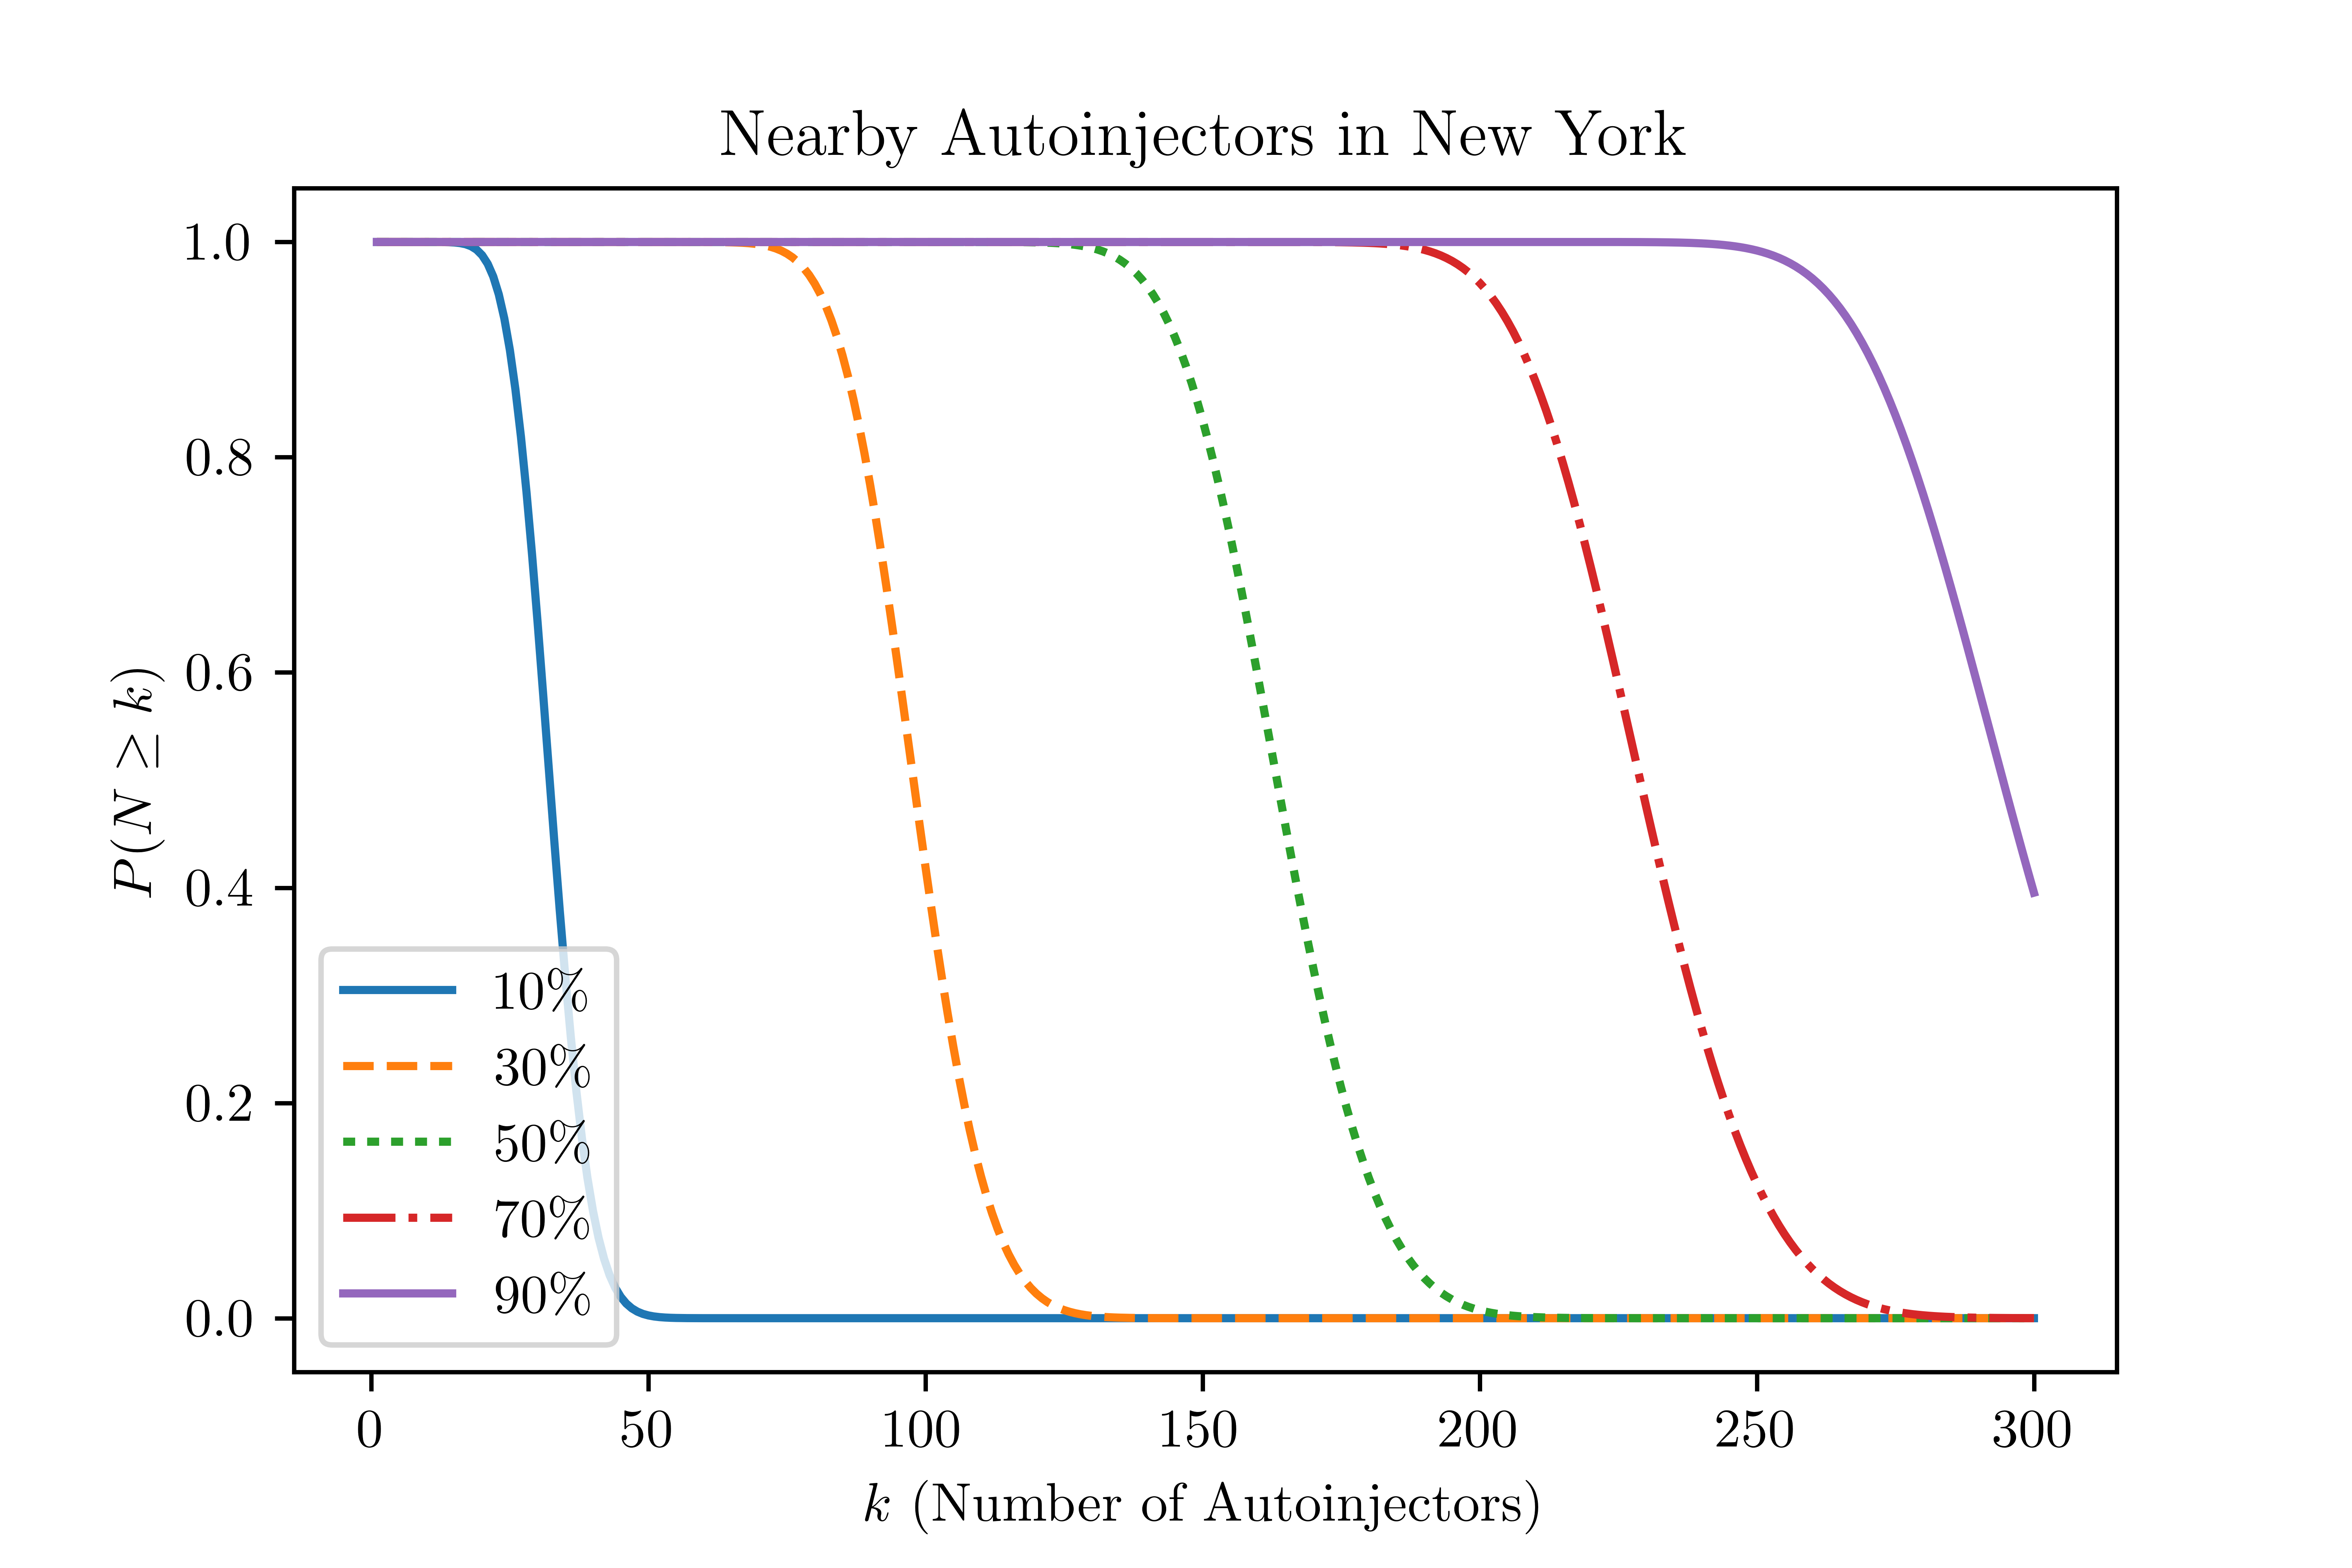
\includegraphics[width=\linewidth]{NewYork-cmfs}
%  \caption{A subfigure}
  \label{fig:newyorkcmf}
\end{subfigure}%
\begin{subfigure}{.5\textwidth}
  \centering
  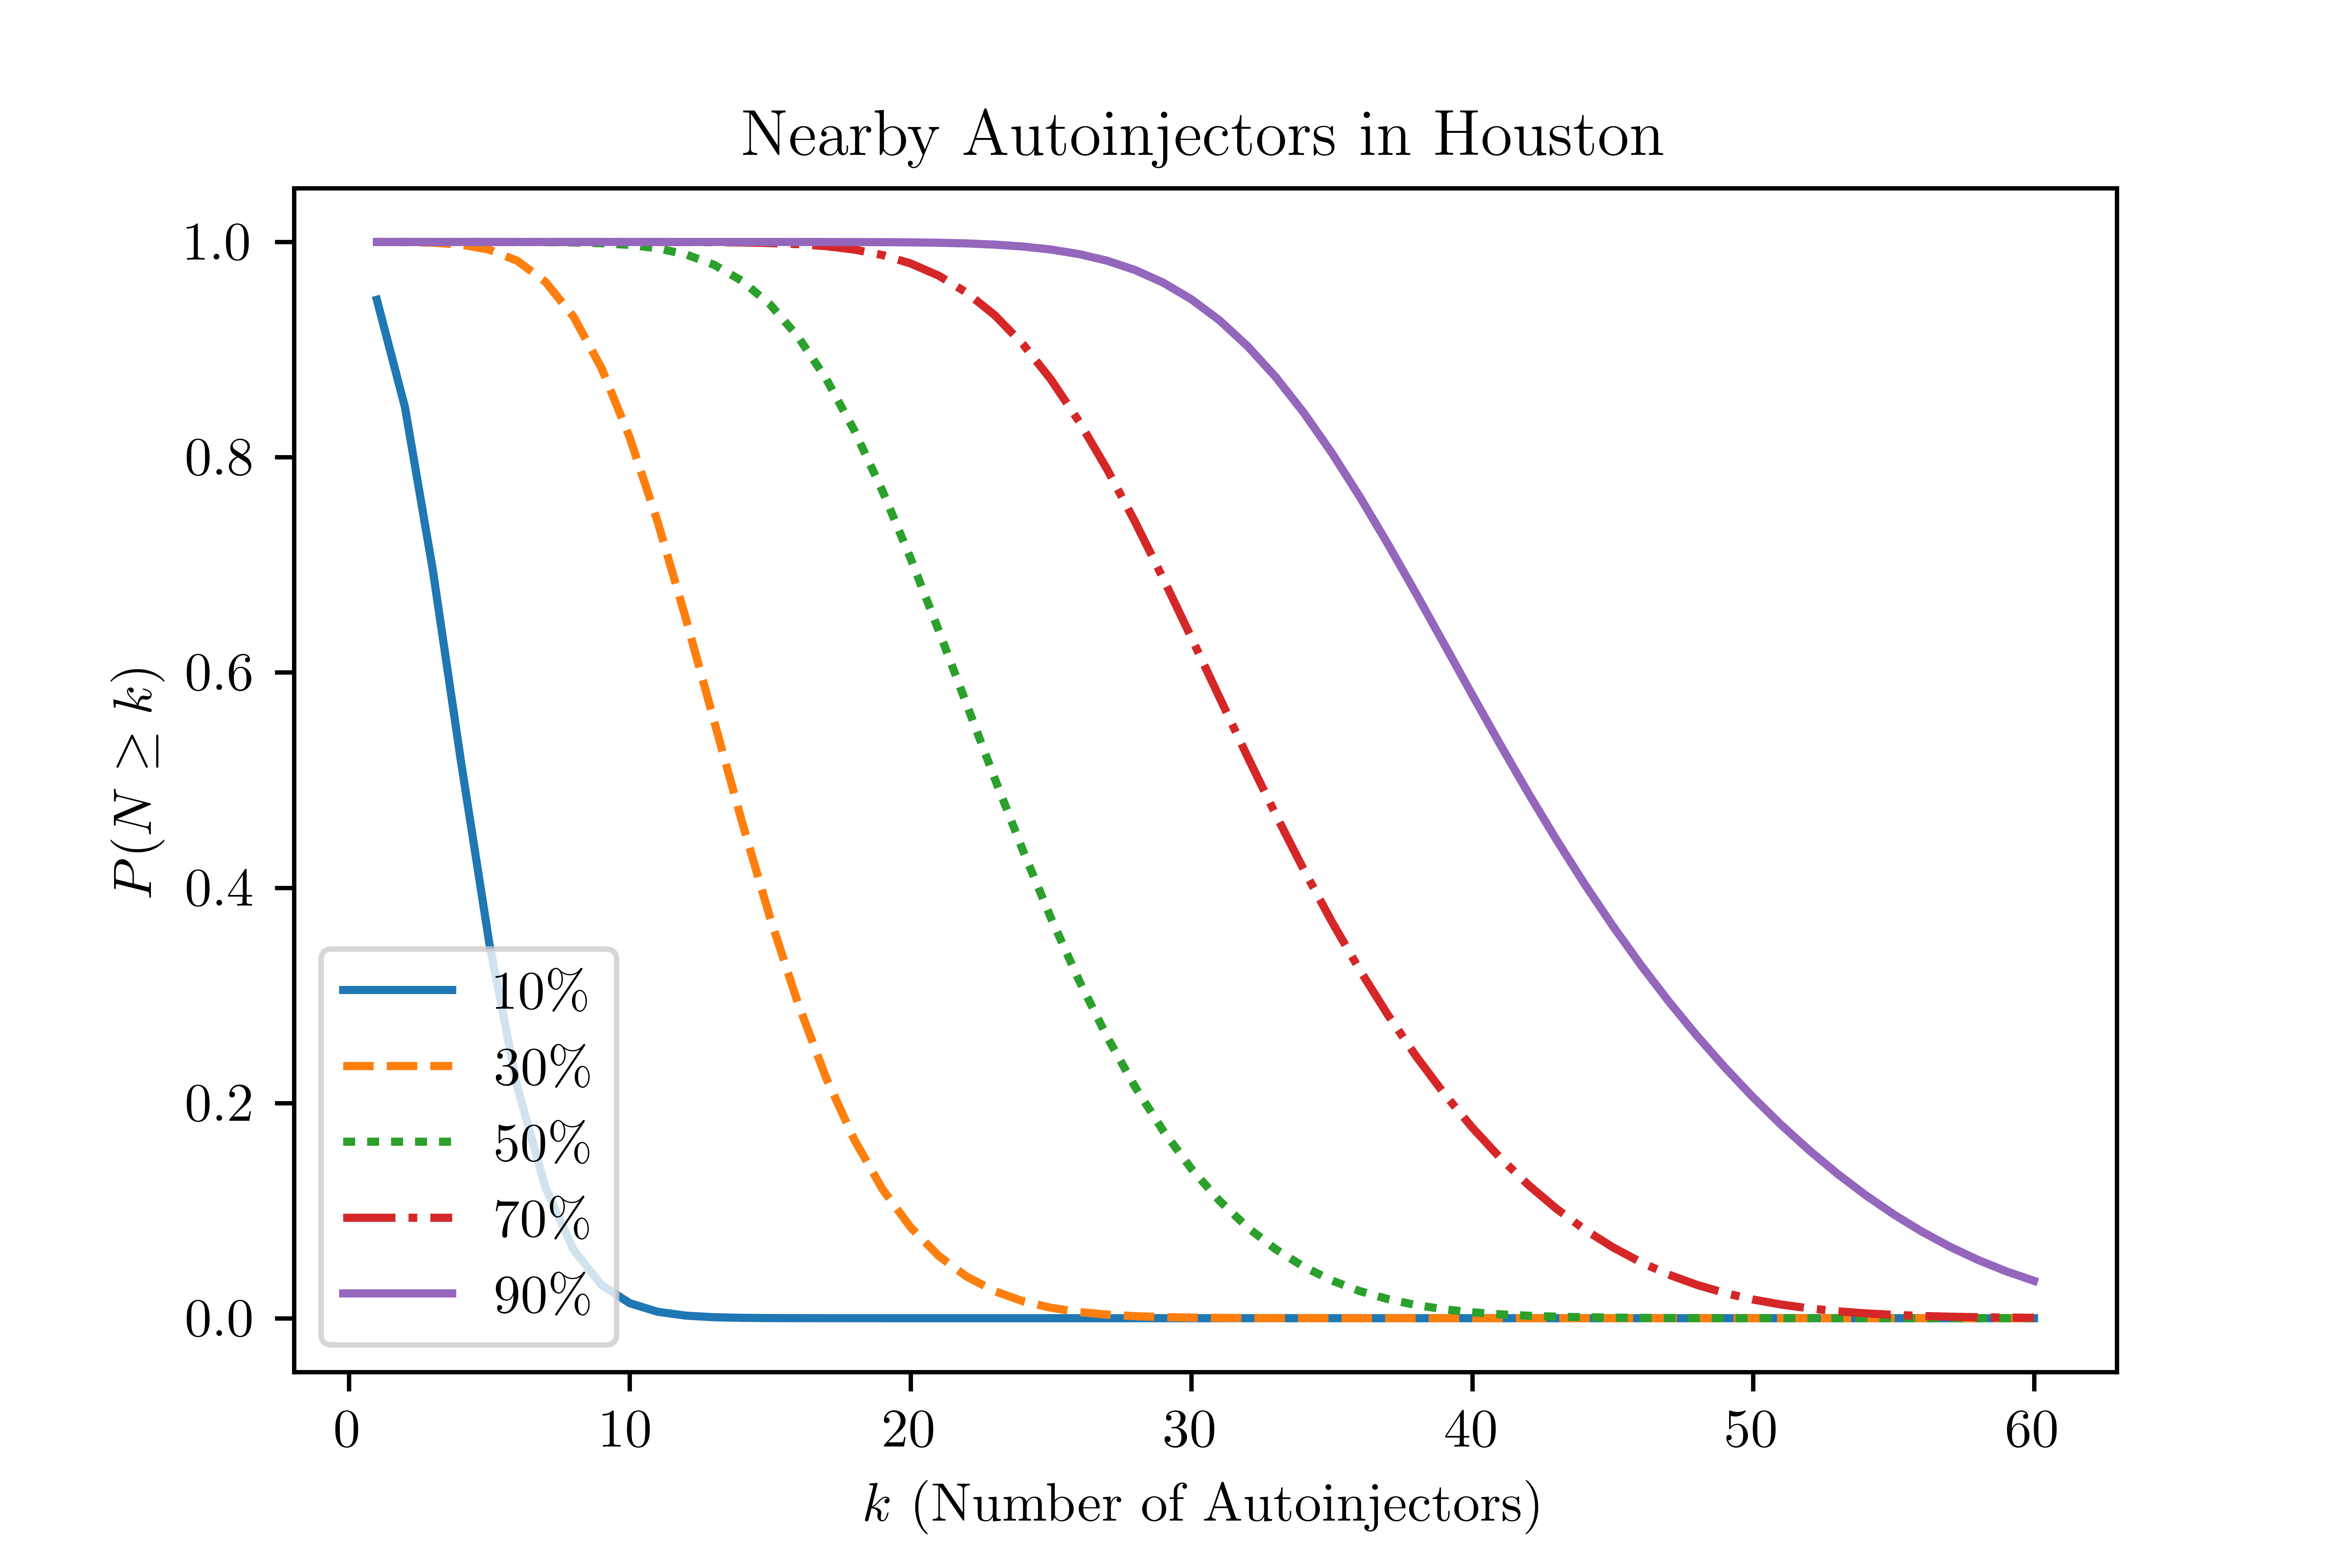
\includegraphics[width=\linewidth]{Houston-cmfs}
%  \caption{A subfigure}
  \label{fig:houstoncmf}
\end{subfigure}
\caption{$P(N\geq k)$ for New York City and Houston. Each line represents a different value for $P(C)$, ranging from 10\% to 90\%.}
\label{fig:nyandhouston}
\end{figure}
As can be see, a higher population density corresponds to an increase in the expected number of autoinjectors neraby. As shown in Figure \ref{fig:nyandhouston}, even if 50\% of people with autoinjector prescriptions carry it on their person, there is only a 50\% chance there will be at least 25 autoinjectors nearby in Houston compared to New York's 160. New York and Houston are the first and fourth largest populated cities in the U.S. respectively \cite{acs}, yet there is a significant difference in likelihood due to their differing populatino densities. We next consider this effect more formally and determine the number of people living in different population densities in the U.S. and the resulting effect on $P(N \geq k)$.

\subsection{Population Densities}

As shown in Section \ref{autoinjectors-nearby} through the cities of New York and Houston, a higher population density corresponds to an increase in the expected number of autoinjectors nearby. Figure \ref{fig:denscomp} shows this effect of population density on $P(N\geq k)$ for two different values of $P(C)$. As expected, the probability of having an autoinjector nearby is proportional to population density. 

\begin{figure}[h]
\centering
\begin{subfigure}{.5\textwidth}
  \centering
  \includegraphics[width=\linewidth]{{{dencomp-pc-0.3}}}
%  \caption{A subfigure}
  \label{fig:den03}
\end{subfigure}%
\begin{subfigure}{.5\textwidth}
  \centering
  \includegraphics[width=\linewidth]{{{dencomp-pc-0.5}}}
%  \caption{A subfigure}
  \label{fig:den05}
\end{subfigure}
\caption{Comparing $P(N\geq k)$ for different population densities. As the population density increases, the chances of having more autoinjectors nearby increases. The graph on the left assumes $P(C) = 0.3$ while the right assumes $P(C) = 0.5$. The units of population density, $\rho$, is people/km$^2$.}
\label{fig:denscomp}
\end{figure}

An important consideration that arrises from this analysis is determining how many people in the U.S. live in an area with a population density that allows a reasonable probability of having an autoinjector nearby. If the number is too low, then an implementation of this network might not be fiscally practical. Figure \ref{fig:popbydensity} shows $uP(T)P(C)$---the number of people in the U.S. population that live have prescriptions for autoinjectors and carry them on their person---living in different population densities. The y-axis shows the number that live in an area of at least the density of the value on the x-axis.

\begin{figure}[h]
\centering
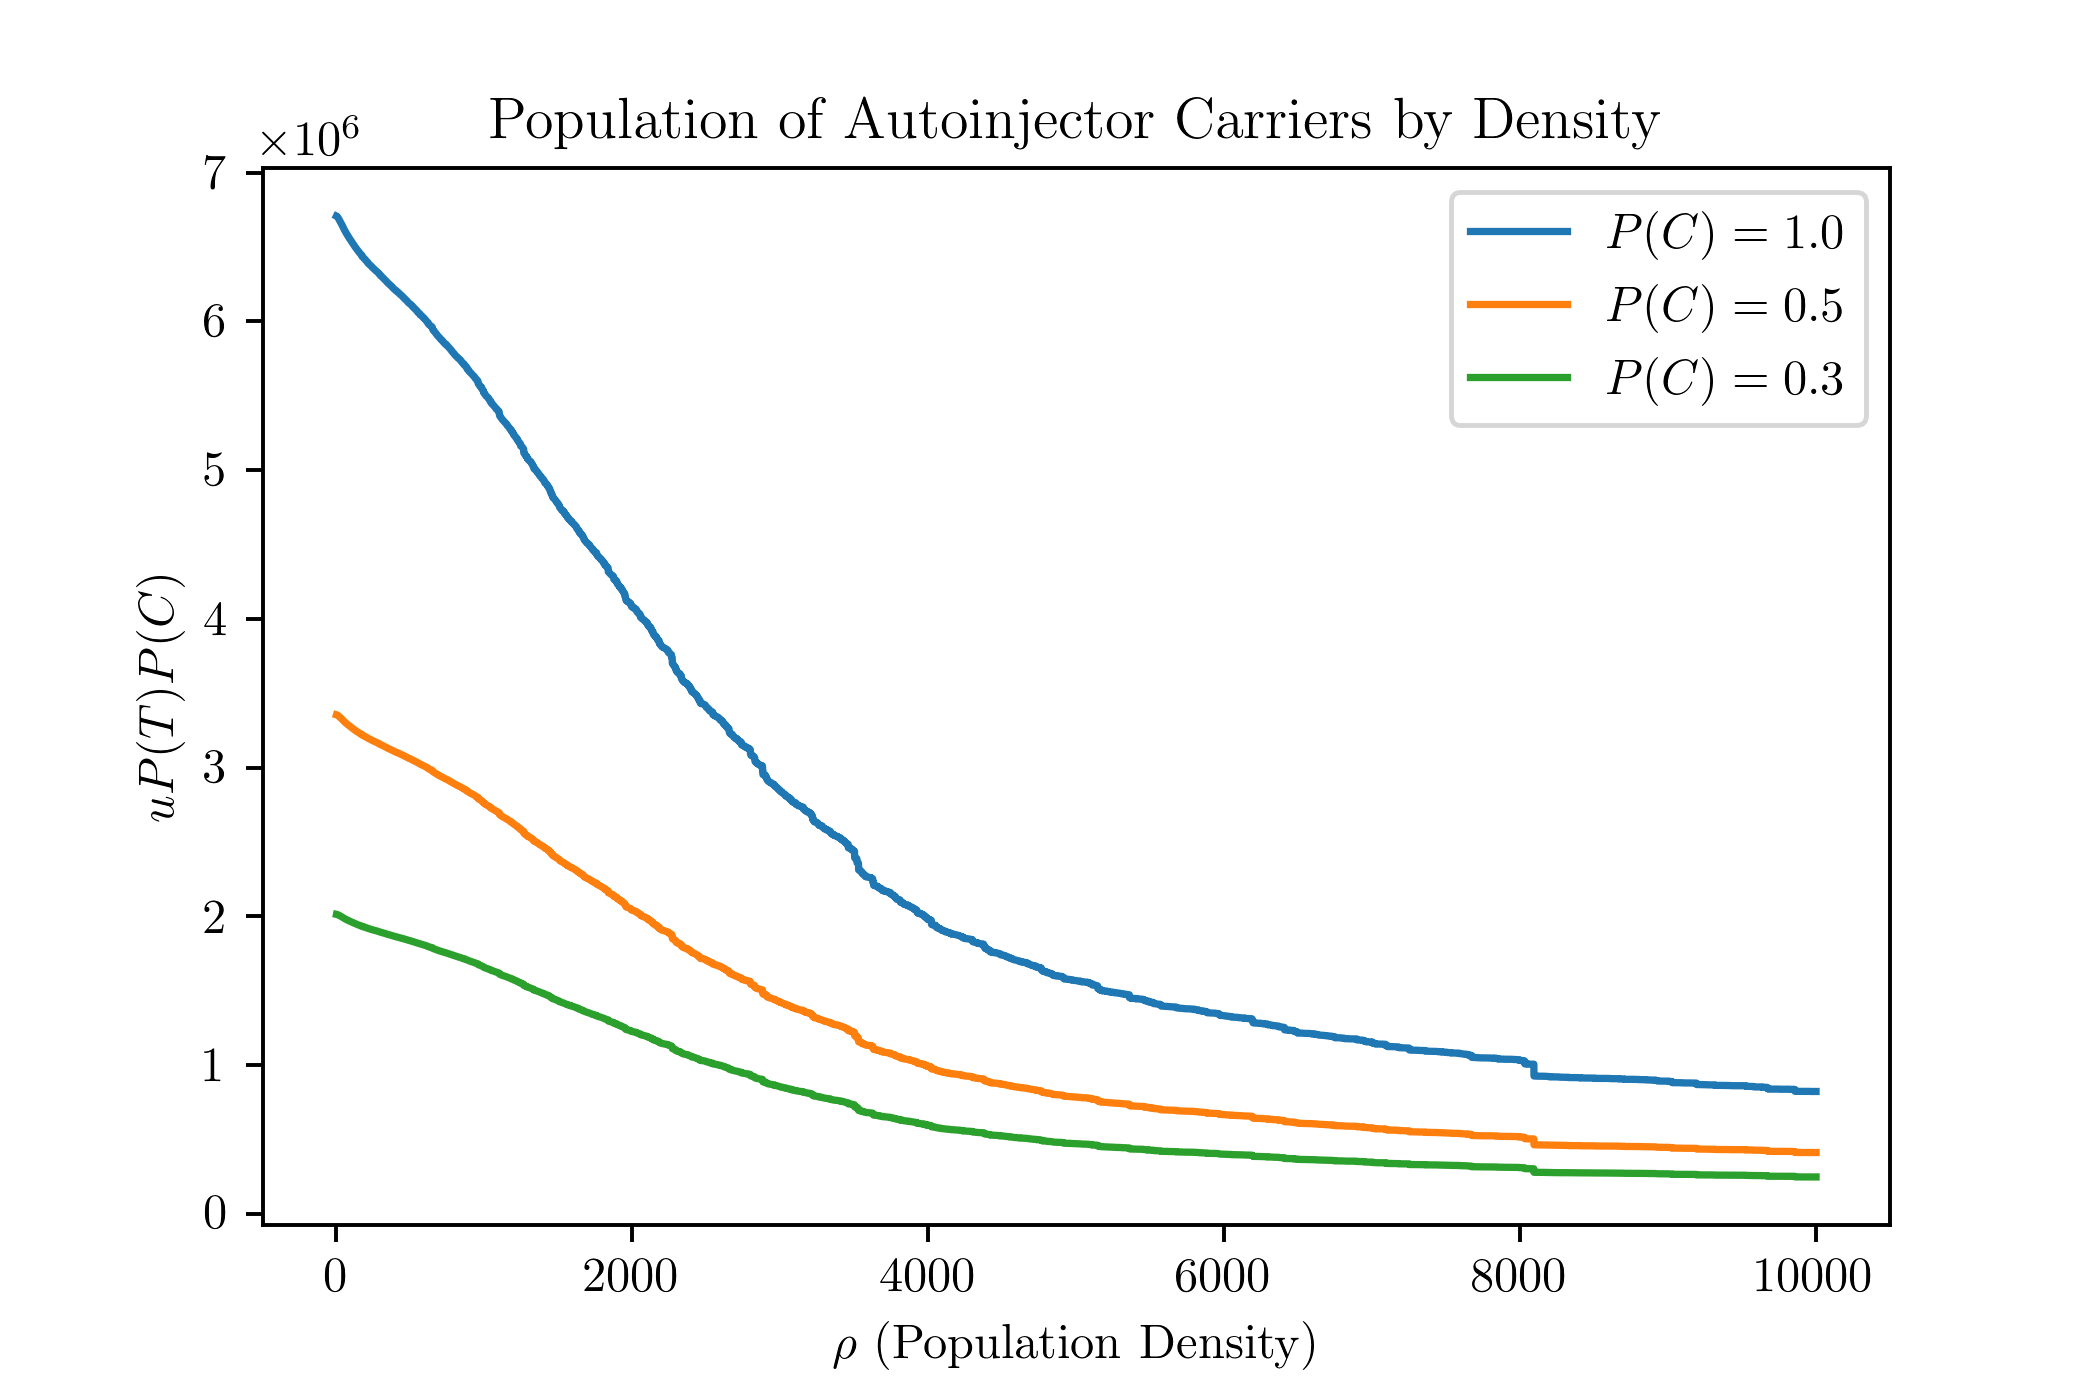
\includegraphics[width=0.5\textwidth]{popbydensity}
\caption{Population of autoinjector carriers that live in areas of differing population densities. The y-axis shows the number of autoinjector carriers that lives in an area of at least the density of the value on the x-axis.}
\label{fig:popbydensity}
\end{figure}

The relationship between Figures \ref{fig:denscomp} and \ref{fig:popbydensity} combine to show how many autoinjector prescribers live in areas where $P(N \geq k) > 0.5$ for different values of $k$. These results are shown in Table \ref{tab:probsforks}. Recall that $P(C) = 1.0$ means that everyone with an autoinjector carrying it on their person, and thus $uP(T)P(C)$ represents the total number of people with autoinjector prescriptions. Thus, for any value of $k$ in Table \ref{tab:probsforks}, $uP(T) : P(N\geq k) > 0.5$ indicates of the total number of people \textit{who might need} an autoinjector in living in areas where $P(N \geq k) > 0.5$. As can be seen, over 6 million people who might need an autoinjector live an area where it is more likely than not that there are at least 10 autoinjectors within walking distance if at least 30\% of prescribers are carrying their autoinjector.

\begin{table}[h]
\centering
\begin{tabular} {|c||c|c|}
    \hline
    & \multicolumn{2}{|c|}{$uP(T) : P(N\geq k) > 0.5$} \\\hline
    $k$ & $P(C) = 0.3$ & $P(C) = 0.5$ \\\hline\hline
    10 & $6.06 \times 10^{6}$ & $6.31 \times 10^{6}$ \\\hline
    20 & $4.89 \times 10^{6}$ & $5.09 \times 10^{6}$ \\\hline
    50 & $3.11 \times 10^{6}$ & $3.34 \times 10^{6}$ \\\hline
    90 & $9.89 \times 10^{5}$ & $1.50 \times 10^{6}$ \\\hline 
\end{tabular}
\caption{Population of autoinjector carriers living in areas where the probability of having at least $k$ autoinjectors nearby $P(N \geq k)$, is at least $1/2$ for different values of $k$ and $P(C)$.}
\label{tab:probsforks}
\end{table}

These results indicate that millions of people who might need an autoinjector in an emergency live in areas where a crowdsourcing app could, on average, supply one faster than an ambulance. Based on these results, we can conclude that creating such a crowdsourcing network is indeed possible.

% best link ever https://factfinder.census.gov/faces/tableservices/jsf/pages/productview.xhtml?src=bkmk


%// TODO: Show population densities needed for at least 5, 10, and 20 autoinjectors nearby
%
%// TODO: Show total population of all cities with the population density thresholds above, and expected number of people with food allergies affected
%
%\subsection{Active Users Needed}
%
%// TODO: Show how many active users needed to make it useful
%
%




%Table \ref{top5} shows the probabilities for different $k$ values for the 5 most heavily populated cities in the U.S.

%\begin{table}[h!]
%\begin{center}
%\begin{tabular}{|c|c|c|c|c|c|}
%\hline
%$k$ & New York City & Los Angeles & Chicago & Houston & Philadelphia \\ \hline
%1  & 0.999 & 0.999 & 0.999 & 0.993 & 0.999 \\\hline
%5  & 0.999 & 0.947 & 0.997 & 0.574 & 0.996 \\\hline
%10 & 0.999 & 0.434 & 0.865 & 0.036 & 0.863 \\\hline
%15 & 0.999 & 0.051 & 0.380 & $<0.001$ & 0.493 \\\hline
%30 & 0.768 & $< 0.001$ & $< 0.001$ & $<0.001$ & 0.015 \\\hline
%\end{tabular}
%\end{center}
%\caption{$P(N\geq k)$ for the 5 most heavily populated cities in the U.S.}
%\label{top5}
%\end{table}

%As can be seen in Table \ref{top5}, the probability that there are at least $k$ autoinjectors near Person $X$ declines fairly quickly in these highly populated areas. However, the size of the population is not the critical component; instead, the \textit{population density} is what determines the number of people $n$ in Area $A$.